\chapter{Interactions of ions with phospholipid bilayers}
\label{chap:results}

Biological membranes naturally exist in a weak electrolytic solution of \ce{KCl} on the intracellular side, and of \ce{NaCl} on the extracellular side. 
The biological relevance of these ions reaches from relatively simple osmotic effects to the complex processes in neural signalling. 

Calcium is an important cation in biology, 
which takes part in many signalling pathways and processes, 
e.g., triggering the release of neurotransmitters in neurons, allosterically activating enzymes, 
regulating cardiac rythm in the hearts, and contracting muscles. \citep{Wang2000, Michalak2002, Glancy2013, Chouhan2012, Berridge2003, Clapham2007, Annunziata2013}
The interaction of \ce{Ca^{2+}} with phospholipid membranes has recently recieved attention from both experiments and simulations \citep{melcrova16, javanainen17, catte16, melcr18, magarkar2017, fink2017osmotic, ye2018phosphatidylinositol}.

% Pavel suggested removing this whole paragraph, as it only recaps previously written sections
%In the previous chapter, we presented new classical MD models of phospholipids,
%which account for electrionic polarization via ECC (introduced in section~\ref{section:ecc}). 
%It was demonstrated that ECC-lipids 
%meet current accuracy standards in the field 
%achieved by matching them against X-ray diffraction data and 
%NMR order parameters at various concentrations of salts (section~\ref{section:ecc-lipids}). 
%The effects of electronic polarization are crucial for an accurate response of lipid head group order parameters 
%with respect to an increasing amount of charge bound to the membrane, 
%which was used during the development of the model 
%as will be shown in the following sections. 


In this chapter, we will provide a detailed insight into the interactions of these ions with neutral and negatively charged model membranes,
namely with a POPC bilayer and with a negatively charged bilayer with the composition of 5~POPC:1~POPS. 
We employ our newly developed models of ions and phospholipids, 
i.e.,
ECC-ions \citep{martinek17, kohagen16, Pluharova2014} and ECC-lipids \citep{melcr18}, 
which provide a major improvement over any state-of-the-art model of ions or lipids in terms of lipid-ion interactions. 

First, we summarize the literature knowledge on the interactions of ions with membranes in experiments and simulations.
Then, we demonstrate the accuracy of the newly developed lipid models from ECC-lipids
by showing the response of the head group order parameters to a membrane-bound charge.
%validating ECC-POPC as an accurate model of the lipid electrometer. 
At last, we will provide detailed insight into the binding of cations to the neutral and negatively charged bilayers. 
We put extra emphasis on the interactions with \ce{Ca^{2+}}, 
for which we present the first simulation results that are in \emph{quantitative} agreement with experiments. \citep{catte16, melcr18}






\section{Binding of cations to phospholipid bilayers and lipid electrometer concept from experiments and simulations}
\label{section:electrometer_exp_sim} 

The response of the head group order parameters 
to a given amount of bound charge in the bilayer 
was calibrated using monovalently charged surfactants in \citep{scherer89, akutsu81, altenbach84}. 
After such a calibration,
binding affinities of free cations can be estimated from the measured head group order parameter changes. \citep{scherer89}
This forms the lipid electrometer concept (introduced in section\ref{section:electrometer}),
which can be used to directly compare experimental measurements with MD simulations. 
We performed such a comparison for both neutral and negatively charged membranes 
in \ce{NaCl} and \ce{CaCl2} aqueous solutions using a large set of MD simulations 
produced within NMRlipids open collaboration platfrom \citep{nmrlipids}. 
It was concluded  that the binding affinities of cations are overestimated in almost all models studied in~\citep{catte16} (Fig.~\ref{fig:catte16}) and Ref.~\citep{nmrlipids_proj4}). 


The small head group order parameter response of a neutral POPC bilayer to \ce{NaCl} from the experiments by~\citet{seelig87} is captured by only a few models, 
namely Lipid14 \citep{dickson14}, 
Orange \footnote{See supplementary infromation in \citep{catte16} for further information about the model Orange.} 
and CHARMM36 \citep{klauda10}. 
However, the experimentally measured head group order parameter response to \ce{CaCl2} is not reproduced quantitatively by the models. \citep{catte16}
In addition, none of the employed models in that study reproduces the order parameters without any salt concentration
within experimental error, indicating structural inaccuracies of varying severity in all of them~\citep{botan15}.
In summary, all models of a PC bilayer examined in \citep{catte16} 
overestimate the response of head group order parameters and/or binding affinity of \ce{CaCl2} to such bilayers. 



\begin{figure}[tbp]
  \centering
  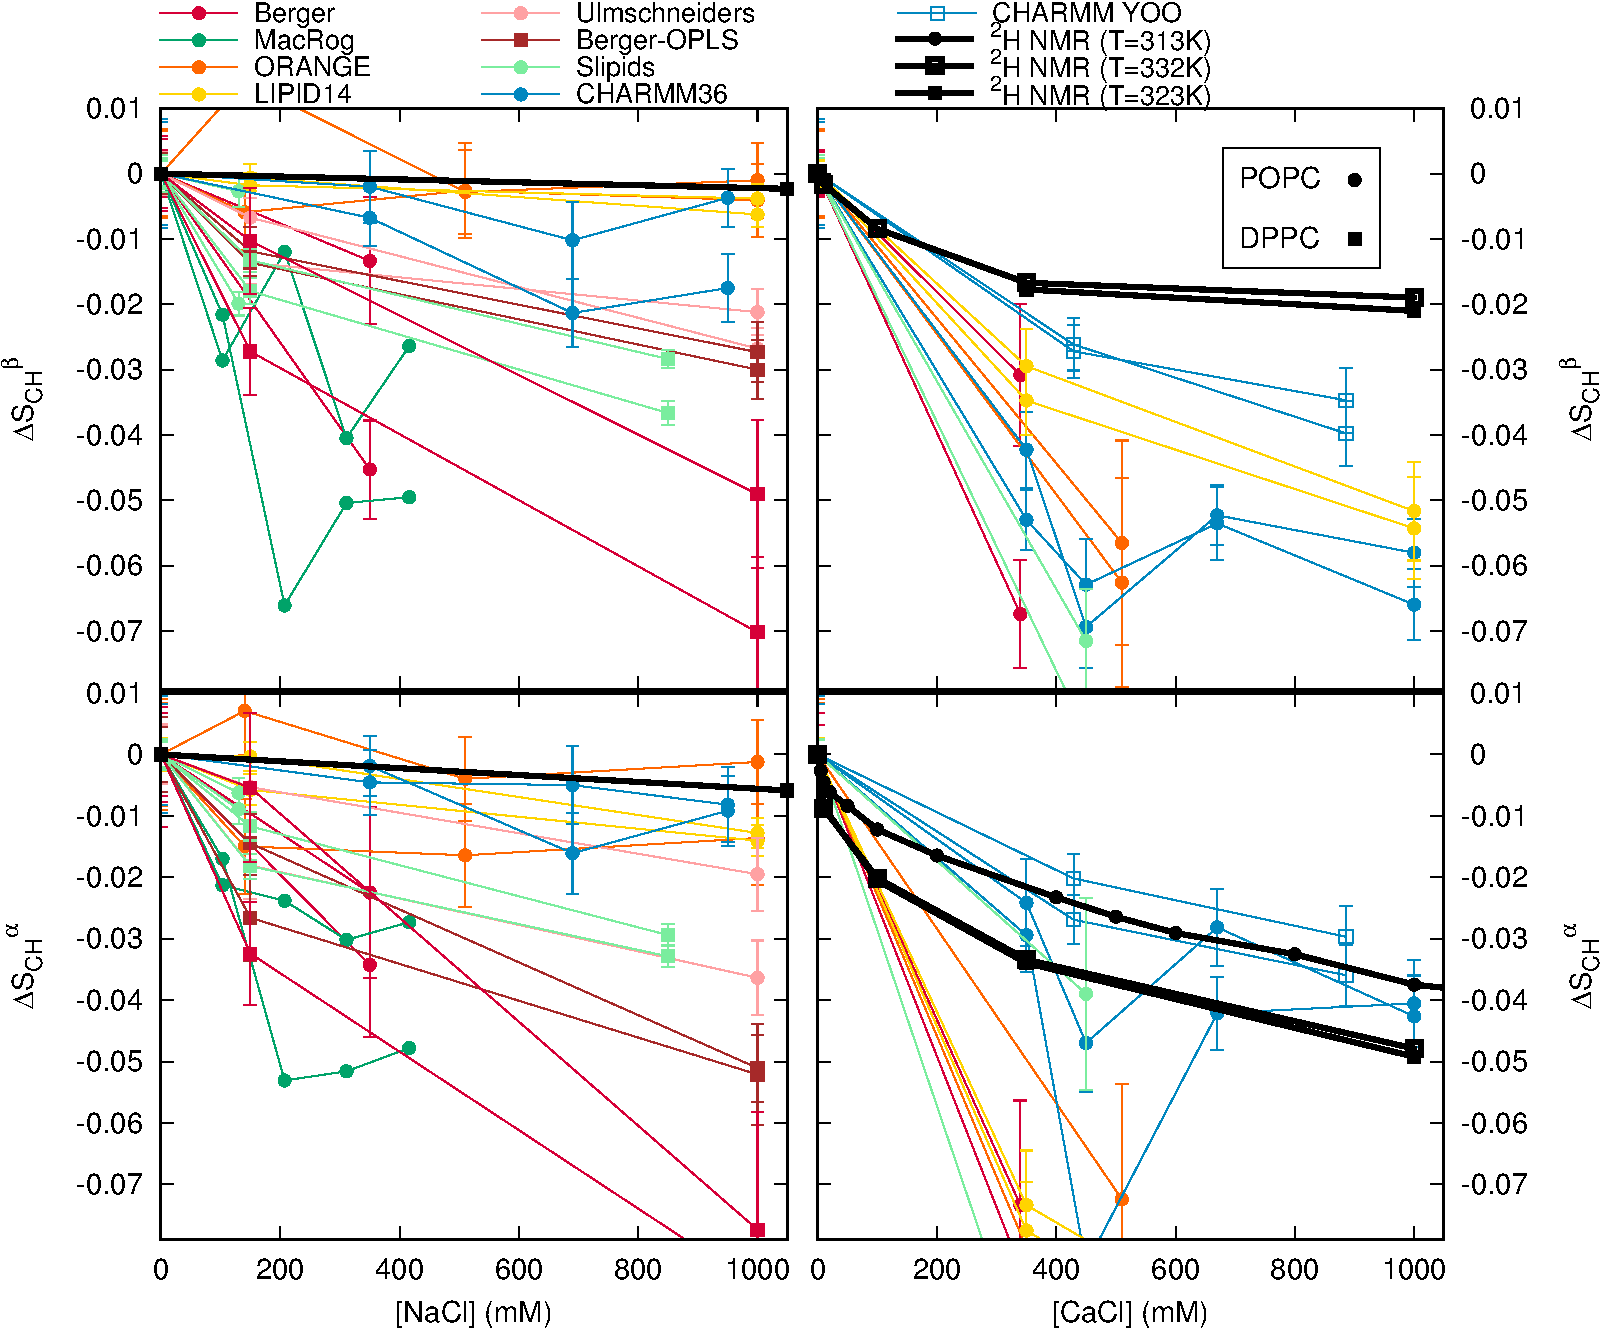
\includegraphics[width=\figwidthfull]{../img/OrderParameterIONSchanges.pdf}
  \caption{\label{fig:catte16}
    Changes of the head group order parameters $\beta$ (top row) and $\alpha$ (bottom row) 
    to increasing concentrations of \ce{NaCl} (left column) and \ce{CaCl2} (right column)
    Results from experiments 
    (DPPC from Ref.~\citep{akutsu81}, POPC from Ref.~\citep{altenbach84}) 
    are compared with simulations with different force fields \citep{nmrlipids, catte16}. 
    Note that none of the employed models in this figure reproduces the order parameters without any salt concentration
    within experimental error, indicating structural inaccuracies of varying severity in all of them~\citep{botan15}.
  }
\end{figure}


Similar conclusions to those from neutral POPC bilayers 
are also reached for negatively charged membranes containing POPS \citep{nmrlipids_proj4}. 
The structure of a POPS bilayer with only \ce{Na^+} counterions
is not captured within the experimental error by any of the studied model. 
However, the small response of the order parameters of PC and PS head groups 
to incresing concentrations of \ce{NaCl} in a mixed bilayer with the composition 5\,PC:1\,PS 
is captured by a few, 
namely Lipid17 \citep{lipid17-future} and less well in MacRog \citep{maciejewski14}. 

Interestingly, the response to \ce{CaCl2} is overestimated by all employed models but one, 
CHARMM36 obtained from \url{http://charmm-gui.org/} \citep{jo08, lee15},
which contains an ad hoc correction for the observed excessive binding of \ce{Ca^{2+}} to PC and PS similar to the correction for \ce{Na^+} \citep{venable13}. 
With such a model, the response of the head group order parameters of PC 
to increasing concentrations of \ce{CaCl2} in a mixed negatively charged bilayer
is significantly reduced by the employed correction for \ce{Ca^{2+}}, 
even below the response measured experimentally. 
Hence, it is the only model in the study,
which underestimates the response of the lipid electrometer for the negatively charged membrane. 
This is in stark contrast to the results from the neutral POPC bilayer in \citep{catte16}, 
where the ad hoc repulsive correction for \ce{Ca^{2+}} was not yet present.



\begin{figure}[tb!] 
  \centering 
  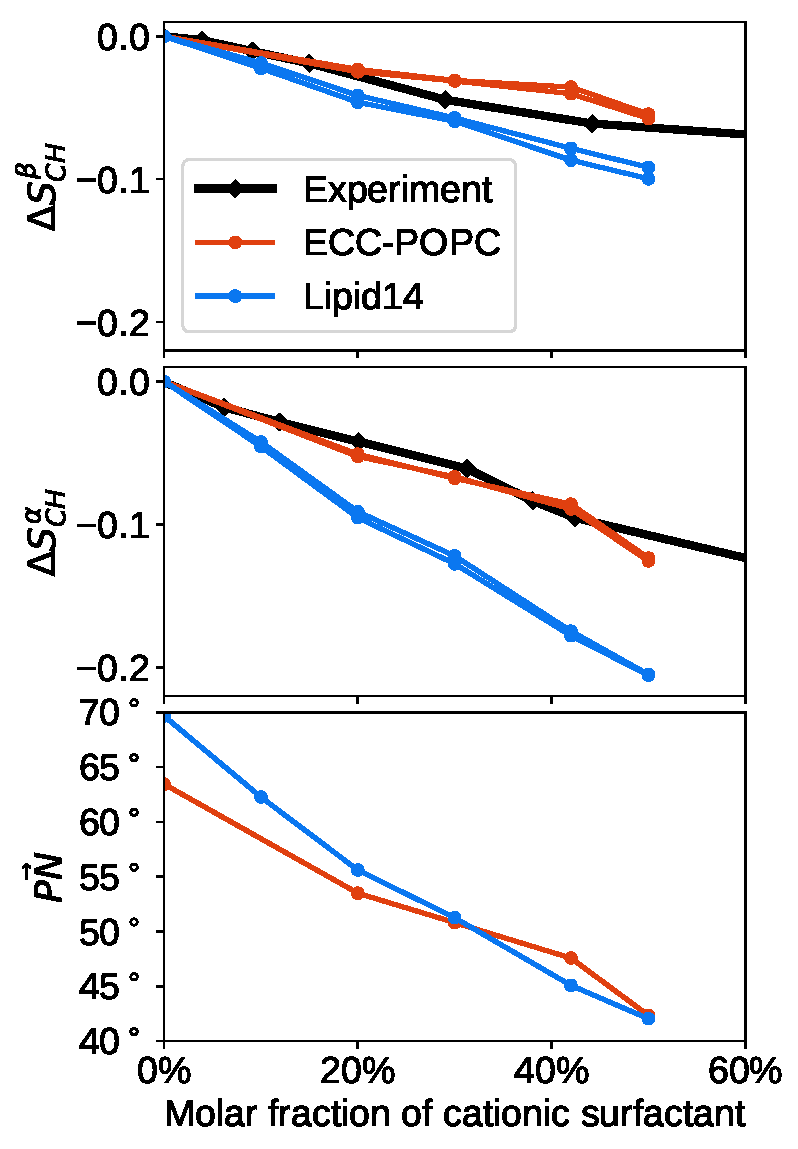
\includegraphics[width=\figwidth]{../img/ecc_popc/PN_angle_OrdPars-A-B_L14-ECCL17_q80_sig89_surf.pdf} 
  \caption{\label{OrderParameterCHANGESsurf} 
    Changes of the head group order parameters $\alpha$, $\beta$ and P-N vector orientation as a function of 
    the molar fraction of a cationic surfactant dihexadecyldimethylammonium in a POPC bilayer 
    from simulations and experiments \citep{scherer89} at 313 K.
  } 
\end{figure} 

 

In order to distinguish, whether the observed discrepancy of the head group order parameter changes between simulations and experiments 
arises from an incorrect sensitivity of the head group or from an excessive binding of cations to the phospholipid bilayers,
we performed simulations of a neutral POPC bilayer with varying amounts of a cationic surfactant dihexadecyldimethylammonium, 
as was measured in the experimental work by \citet{scherer89}.
The amount of bound charge per lipid
in such systems is given simply by the molar fraction of the cationic surfactants, 
as essentially all of the surfactants segregate to the lipid bilayers 
due to the two long hydrophobic tails.
The NMR measurements of such systems  
can be used to validate the sensitivity of lipid headgroup order parameters 
(i.e., the coefficient $m_i$ in Equation~\ref{OPchangeEQ}) 
to the amount of bound charge in simulations. 

The changes of the headgroup order parameters in a POPC bilayer with an increasing amount of 
the cationic surfactant from simulations and experiments~\citep{scherer89} are shown in Fig.~\ref{OrderParameterCHANGESsurf}.
In line with Equation~\ref{OPchangeEQ},
experiments as well as both MD simulation models show an approximately linear decrease of the head group order parameters $\alpha$ and $\beta$.
%Results from simulations with two models are shown.
%We employ our newly developed model ECC-POPC, introduced in the previous chapter, 
%which accounts for electronic polarizability using ECC \citep{leontyev14}.
%For a direct comparison, we also show results for Lipid14, a standard model by \citet{dickson14},
%which served as a starting point in the development of ECC-POPC. 
%This model was also used in the works \citep{catte16, nmrlipids_proj4}. 
The slope of the response of the order parameters %$\alpha$ and $\beta$ 
from the simulation with the ECC-POPC model 
is in a very good agreement with the experiments, 
whereas the slope from the simulations with Lipid14 is too steep. 
This shows that the overestimated response in the work \citep{catte16}
arises at least in part from an excessively sensitive response of the head group. 

The increasing amount of the cationic surfactant in the bilayer
also affects the P-N vector, 
which is defined as the angle between the connector of the phosphorus and nitrogen atoms and the membrane normal. 
Similarly to the order parameters, 
there is a linear dependence on the amount of the cationic surfactant
as shown in Fig.~\ref{OrderParameterCHANGESsurf}. 
Although the structure of the ECC-POPC model without any ions does not agree with NMR experiments within error bars,
such a model reproduces well the changes of the order parameters.
It follows from these observations that using this model
we can write an approximate relation between the changes of the order parameters and the P-N vector mean orientation. 
For the change of the order parameter $\alpha$, $\Delta S^\alpha$, we arrive at
\begin{equation}
\Delta \vec{PN} = (186 \pm 9) \cdot \Delta S^\alpha .
\end{equation}
This relation can be used to estimate the change of the P-N vector as a mean orientation of the head group
from experimental measurements of the change of the order parameter $\alpha$ in POPC. 

%After reproducing the concept of a lipid electrometer with a known amount of bound surface charge,
%ECC-lipids will be employed in the study of interactions with aqueous ions, namely with \ce{K^+}, \ce{Na^+} and \ce{Ca^{2+}}. 












\section{Interactions of neutral and negatively charged phospholipid membranes with Na$^+$ and K$^+$ cations}
\label{section:lip-ion_k_na}

\begin{figure}[tbp!] 
  \centering 
  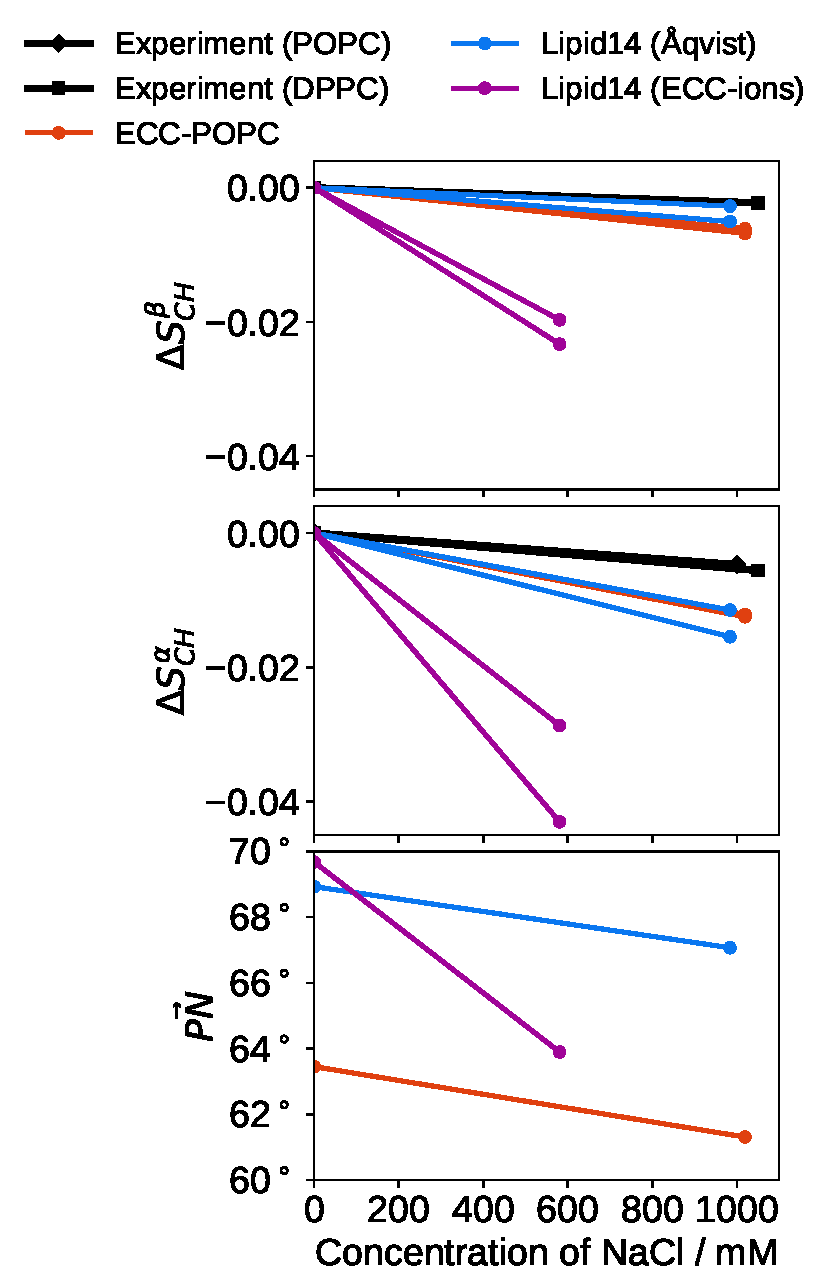
\includegraphics[height=10 cm]{../img/ecc_popc/OrdPars-A-B-PNvec_L14-ECC-lipids_NaCl.pdf}
  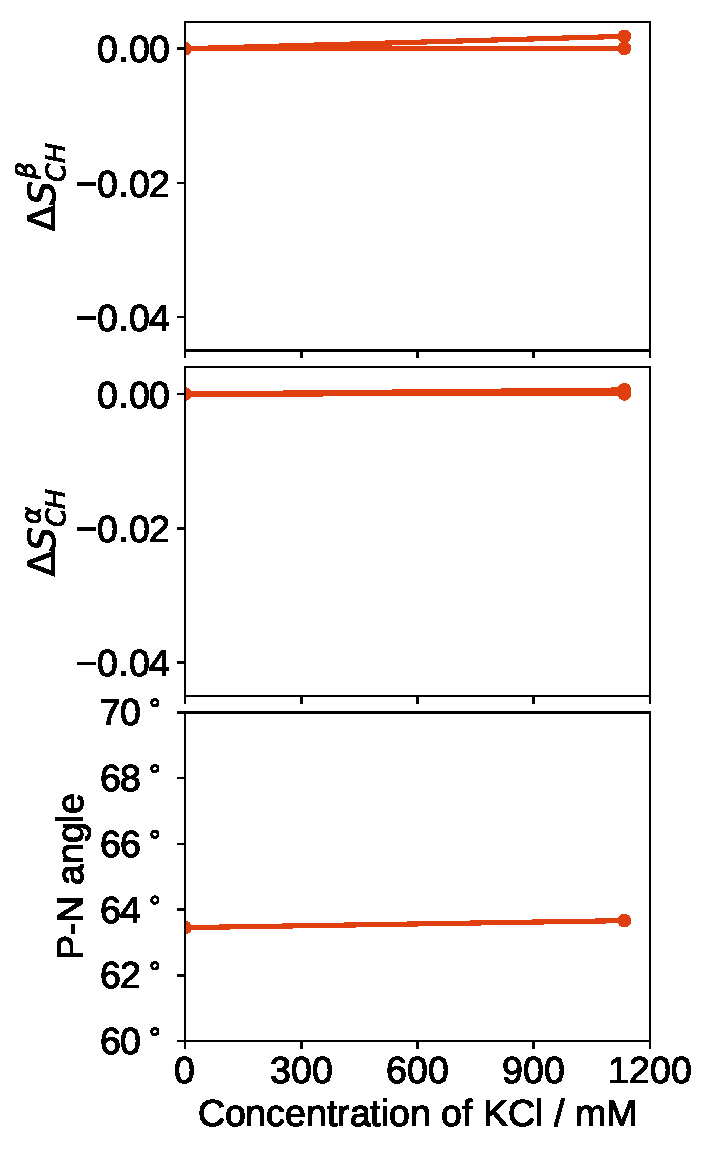
\includegraphics[height= 9 cm]{../img/ecc_popc/OrdPars-A-B-PNvec_L14-ECC-lipids_KCl.pdf}
  \caption{\label{fig:delta_ordPar_NaCl} 
    Changes of head group order parameters $\alpha$ and $\beta$ and P-N vector orientation in a POPC bilayer 
    as a function of \ce{NaCl} (left) and \ce{KCl} (right) concentration 
    in bulk ($C_{ion}$) from simulations with different force fields at 313 K together with  
    experimental data for DPPC (323\,K) \citep{akutsu81} and POPC (313\,K) \citep{altenbach84}. 
    Simulation data with Lipid14 and Åqvist ion parameters at 298 K are taken directly from 
    Refs.~\citep{lipid14POPC0mMNaClfiles,lipid14POPC1000mMNaClfiles}. 
  } 
\end{figure} 
 
 
\begin{figure}[tbp!] 
  \centering 
  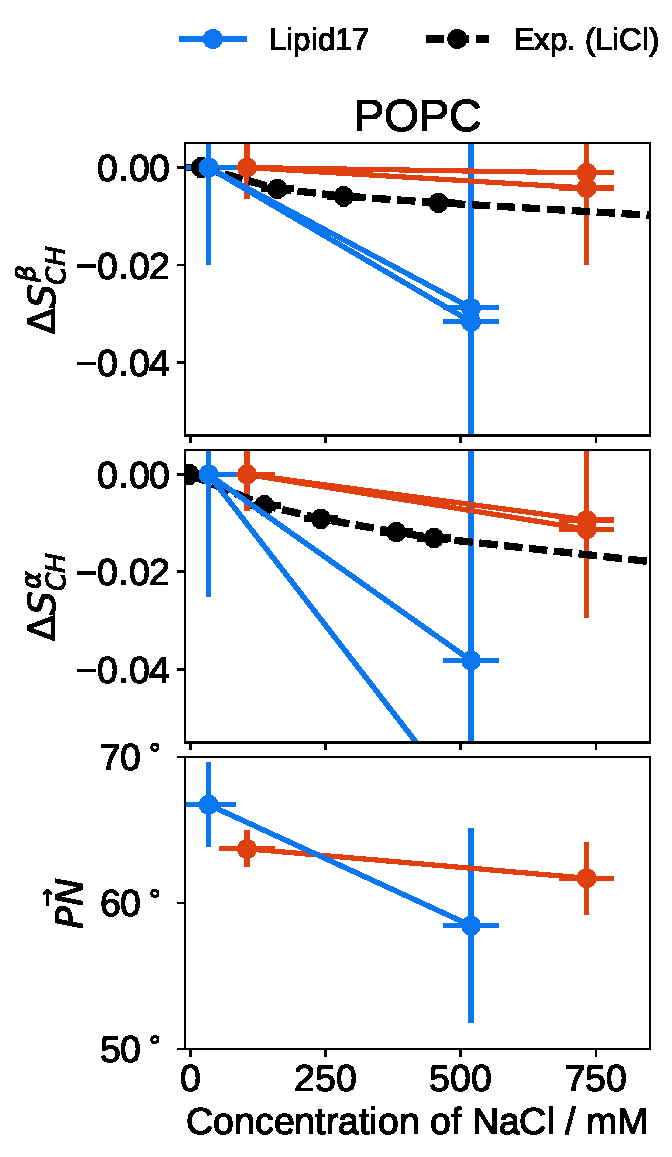
\includegraphics[width=\figwidthsmall]{../img/ecc_pops/order_parameters_changes_ecc-lip_L14_A-B-PN-COO_POPC_nacl.pdf} 
  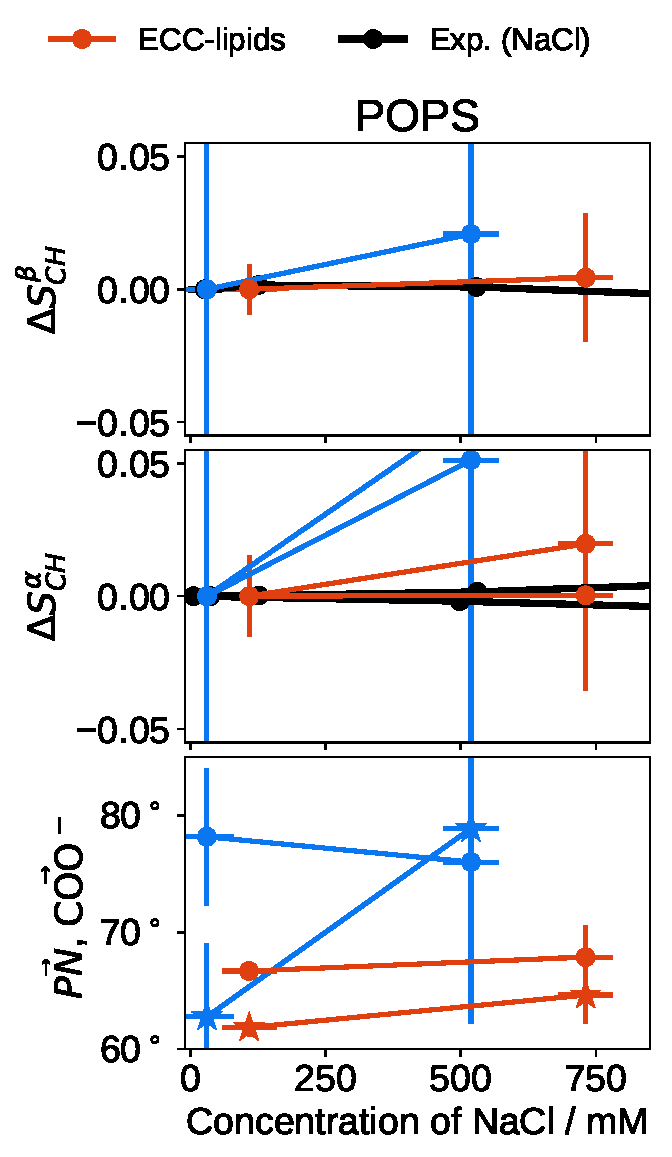
\includegraphics[width=\figwidthsmall]{../img/ecc_pops/order_parameters_changes_ecc-lip_L14_A-B-PN-COO_POPS_nacl.pdf} 
  \caption{\label{fig:delta_ordPar_NaCl_PCPS} 
    Changes of the head group order parameters $\alpha$, $\beta$ and the orientations of the carboxylate group and the P-N vector  
    of POPC (left) and POPS (right) phospholipids in a POPC:POPS 5:1 bilayer as a function of \ce{NaCl} concentration 
    in bulk ($C_{ion}$) from simulations with different force fields at 298 K.
    Because data with \ce{NaCl} are not available for POPC, 
    we show experimental data for \ce{LiCl} (dashed line, left) 
    as an upper bound for the magnitude of the response to \ce{NaCl}, 
    which has a lower affinity to phospholipid bilayers compared to \ce{LiCl} \citep{roux90}. 
    The orientation of the \ce{COO^-} group is defined as 
    the connector from the $\beta$ carbon to the carbon in \ce{COO^-} (stars, bottom right). 
  } 
\end{figure} 


\begin{figure}[tbp!] 
  \centering 
  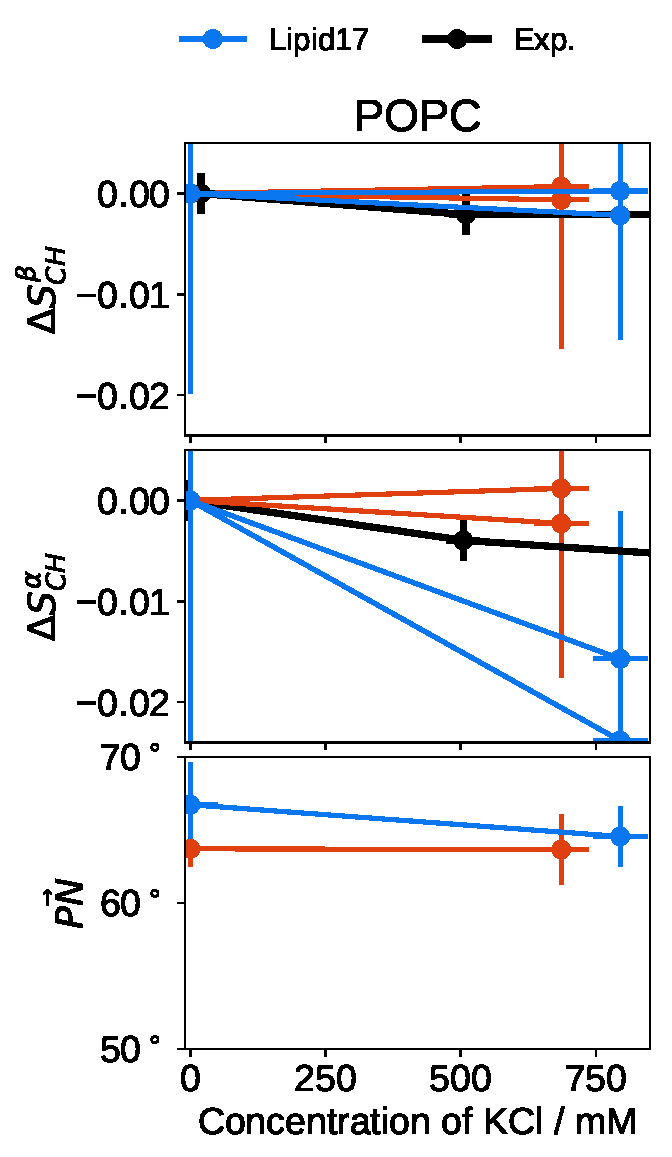
\includegraphics[width=\figwidthsmall]{../img/ecc_pops/order_parameters_changes_ecc-lip_L14_A-B-PN-COO_POPC_kcl.pdf} 
  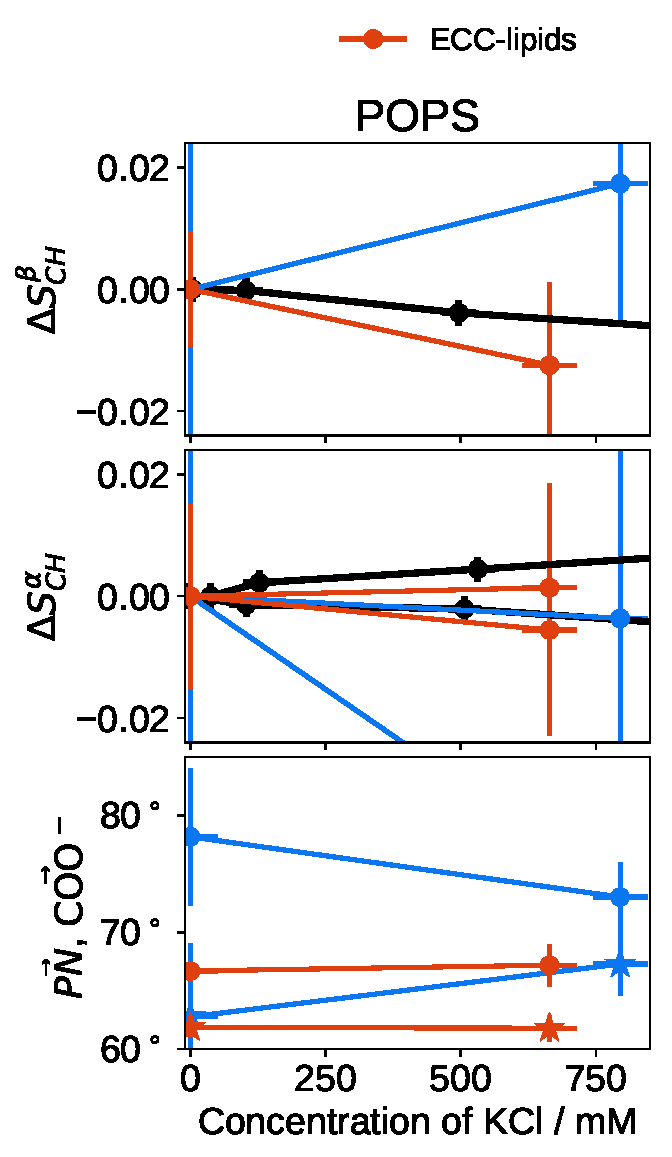
\includegraphics[width=\figwidthsmall]{../img/ecc_pops/order_parameters_changes_ecc-lip_L14_A-B-PN-COO_POPS_kcl.pdf} 
  \caption{\label{fig:delta_ordPar_KCl_PCPS} 
    Changes of the head group order parameters $\alpha$, $\beta$ and the orientations of the carboxylate group and the P-N vector  
    of POPC (left) and POPS (right) phospholipids in a POPC:POPS 5:1 bilayer as a function of \ce{KCl} concentration 
    in bulk ($C_{ion}$) from simulations with different force fields and experiments at 298 K. \citep{roux90}
    The orientation of the \ce{COO^-} group is defined as 
    the connector from the $\beta$ carbon to the carbon in \ce{COO^-} (stars, bottom right). 
  } 
\end{figure} 
 


% Pavel suggested to remove this as it only recaps previous sections
%It was presented in the previous section,
%that accounting for electronic polarization,
%a distinct feature of ECC-lipids compared to other lipid models, 
%is crucial for an accurate description of the response of the POPC electrometer. 
%In this section,
%we employ ECC-lipids to simulate neutral and negatively charged bilayers 
%in the presence of monovalent salts, namely \ce{KCl} and \ce{NaCl}. 

Interactions of \ce{Na^+} with neutral POPC bilayer were studied in \citep{catte16}, 
and with negatively charged mixed 5\,PC:1\,PS bilayer in \citep{nmrlipids_proj4}. 
It was concluded that the interactions are generally overestimated in magnitude in almost all models 
but Lipid14 (PC) \citep{dickson14}, resp. Lipid17 (PS) \citep{lipid17-future}. 
This model yields a semi-quantitative agreement with the experimentally measured small changes of the order parameters 
when used with the model of ions by \citet{aqvist90} (Fig.~\ref{fig:catte16}). 
However, when used with a more accurate model of ions by \citet{Pluharova2014, martinek17},
the model overestimates the binding affinity of \ce{Na^+}
measured with lipid electrometer concept in Fig.~\ref{fig:delta_ordPar_NaCl}. \citep{melcr18}
In line with our previous work \citep{catte16}, the results suggest that improvements 
in the lipid parameters are required for more accurate interactions even with monovalent cations. 

The results from simulations combining the models 
ECC-lipids \citep{melcr18} and ECC-ions \citep{martinek17, kohagen16, Pluharova2014} 
with neutral and negatively charged membranes
exhibit an improved behavior of the POPC and POPS head group order parameters 
as a function of \ce{NaCl} or \ce{KCl} concentrations, 
which is plotted for \ce{NaCl} in Figs.~\ref{fig:delta_ordPar_NaCl}, \ref{fig:delta_ordPar_NaCl_PCPS} 
and for \ce{KCl} in Fig.~\ref{fig:delta_ordPar_KCl_PCPS}. 


The interaction with \ce{K^+}, which binds very weakly to both neutral and negatively charged membranes, 
renders a qualitatively different response of the order parameter $S^\beta$ in POPS in the mixed negatively charged membranes. 
While the order parameter $S^\beta$ increases for both \ce{Na^+} and \ce{Ca^{2+}},
it decreases in the presence of \ce{K^+}.
%This feature is, \emph{qualitatively} captured by a few models in \citep{nmrlipids_proj4},
%neither of them is as close to a \emph{qunatitative} agreement with the experiments 
%as the combination of ECC-lipids with ECC-ions. 
However, no model studied in \citep{nmrlipids_proj4} describes the behaviour of a PS head group correctly enough to reveal this effect. 
In contrast, ECC-lipids with ECC-ions capture the different response of the order parameteres $S^{\beta}$, $S^{\alpha _1}$ and $S^{\alpha _2}$ in POPS to various salts accurately. 
Such a detailed description of the changes of the structural parameters 
demonstrates that including electronic polarization
improves the description of the interactions even for very weakly binding cations like \ce{K^+}. 



\begin{figure}[tbp!] 
  \centering 
  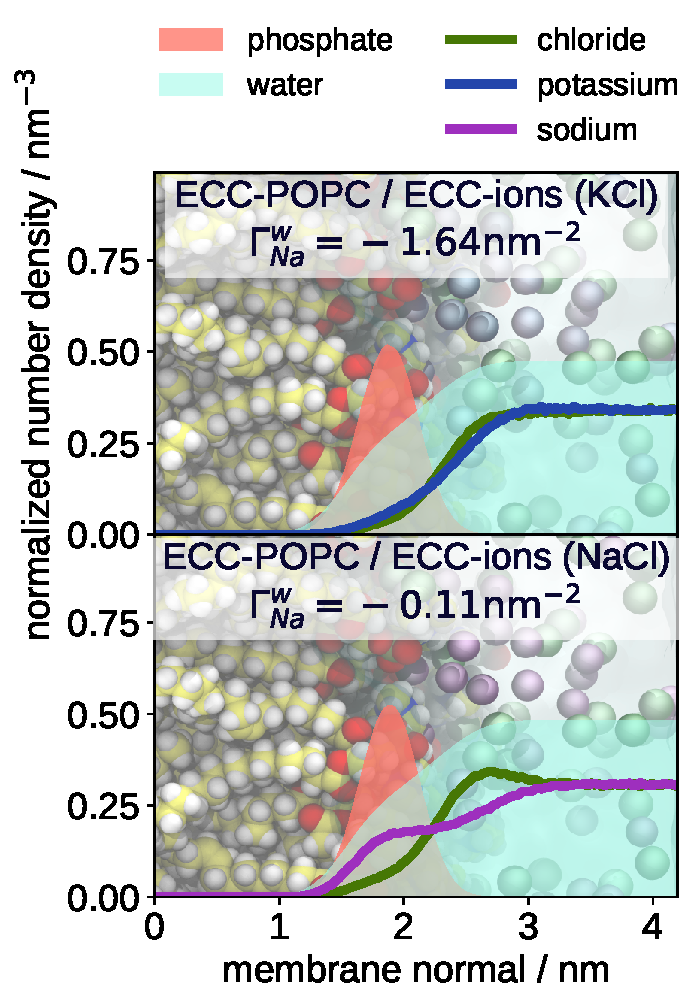
\includegraphics[width=\figwidth]{../img/ecc_popc/density_profiles_ca_cl_wat_phos_models-compar_5-7_NaCl-KCl.pdf}
  \caption{\label{fig:nacl-dens} 
    Number density profiles of \ce{K^{+}}, \ce{Na^{+}} and \ce{Cl^-} along the membrane normal axis 
    from the simulations with the neutral POPC bilayer using ECC-lipids and ECC-ions.  
    In order to visualize the density profiles with a scale comparable to the profile of \ce{Ca^{2+}} in Fig.~\ref{fig:cacl-dens},  
    the density profiles of~\ce{Cl^-}, \ce{K^+} and \ce{Na^+} ions are divided by 2, and 
    the density profiles of phosphate groups and water are divided by 5 and 200, respectively.  
    The simulation with \ce{NaCl} has $C_{ion}'$=1000~mM, 
    the simulation with \ce{KCl}  has $C_{ion}'$=1100~mM. 
    } 
\end{figure} 


\begin{figure}[tbp!] 
  \centering 
  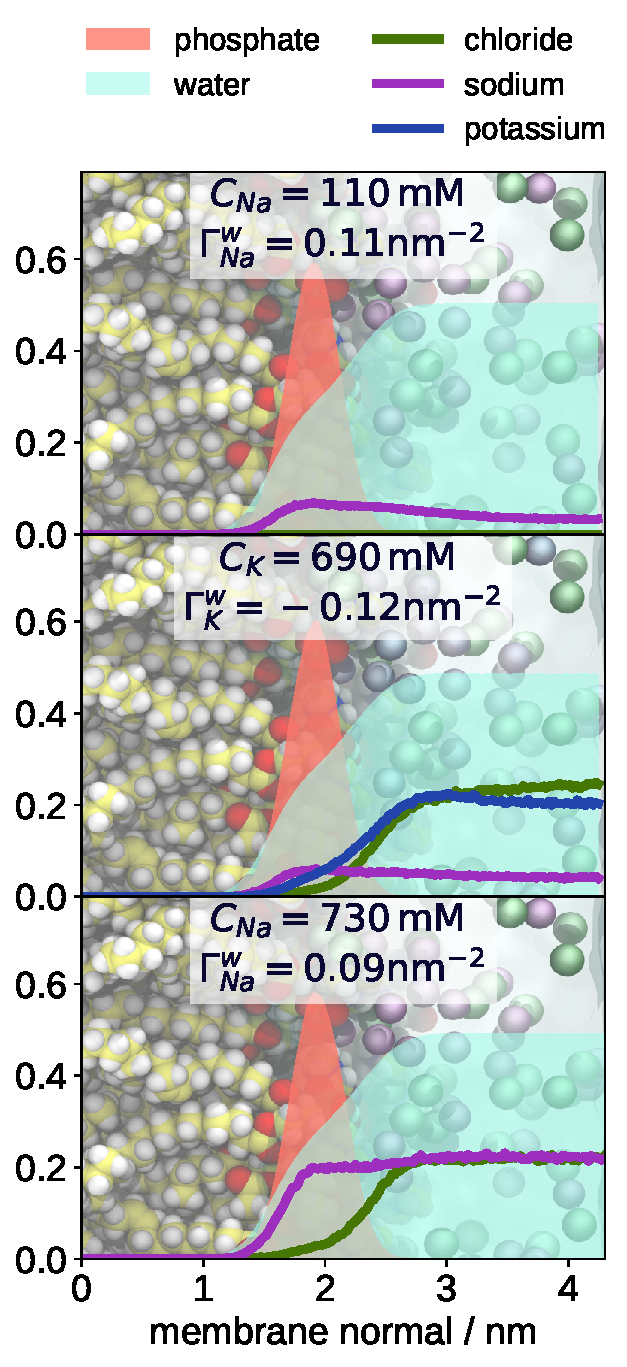
\includegraphics[width=\figwidth]{../img/ecc_pops/density_profiles_na_k_cl_wat_phos_models-compar_4-6_NaCl-and-KCl-series.pdf}
  \caption{\label{fig:nacl-dens_PCPS} 
    Number density profiles of \ce{K^{+}}, \ce{Na^{+}} and \ce{Cl^-} along the membrane normal axis 
    for the negatively charged membrane with the composition of 5\,PC:1\,PS using ECC-lipids and ECC-ions.  
    The top profile shows the simulation without any additional salt concentration, i.e. only with \ce{Na^+} counterions. 
    The middle profile shows the simulation with an additional \ce{KCl} concentration and \ce{Na^+} counterions. 
    The bottom profile shows the simulation with an additional \ce{NaCl} concentration and \ce{Na^+} counterions, which are not distinguished from the added salt. 
    In order to visualize the density profiles with a scale comparable to the profile of \ce{Ca^{2+}} in Fig.~\ref{fig:cacl-dens},  
    the density profiles of~\ce{Cl^-}, \ce{K^+} and \ce{Na^+} ions are divided by 2, and 
    the density profiles of phosphate groups and water are divided by 5 and 200, respectively.  
    } 
\end{figure} 



The difference between the affinities of \ce{Na^+} and \ce{K^+} to neutral and negatively charged membranes
can be described by their relative surface excesses with respect to water, $\Gamma ^{w} _{ion}$, 
which are shown in the plots of the density profiles of the ions in Figs.~\ref{fig:nacl-dens} (neutral bilayer) and \ref{fig:nacl-dens_PCPS} (negatively charged bilayer). 
Such a quantity compares the adsorption of ions to the adsorption of water molecules at an interface 
without the necessity of defining a Gibbs dividing surface. \citep{melcr18, chattorajBOOK}
While \ce{K^+} maintains negative values of $\Gamma^{w}_{K}$ even for the negatively charged bilayer,
the value of $\Gamma^{w}_{Na}$ for \ce{Na^+} changes from negative to positive
in a neutral POPC bilayer versus in a negatively charged bilayer with the composition 5\,PC:1\,PS.
%This means that at the given concentration the bilayer interface has a small preference to \ce{Na^+} cations compared to water molecules. 
Interestingly, this value is slightly decreased in the presence of an additional \ce{NaCl} concentration adding also \ce{Cl^-} anions, 
which are not present in the system when only counterions are used
(bottom resp. top plot in Fig.~\ref{fig:nacl-dens_PCPS}. 
The interaction of a neutral POPC bilayer with \ce{NaCl} is discussed in a greater detail in \citep{melcr18}. 

 





 
 


\section{Interactions of neutral and negatively charged phospholipid membranes with \ce{Ca^{2+}} cations}
\label{section:lip-ion_ca}



\begin{figure}[tbp!] 
  \centering 
  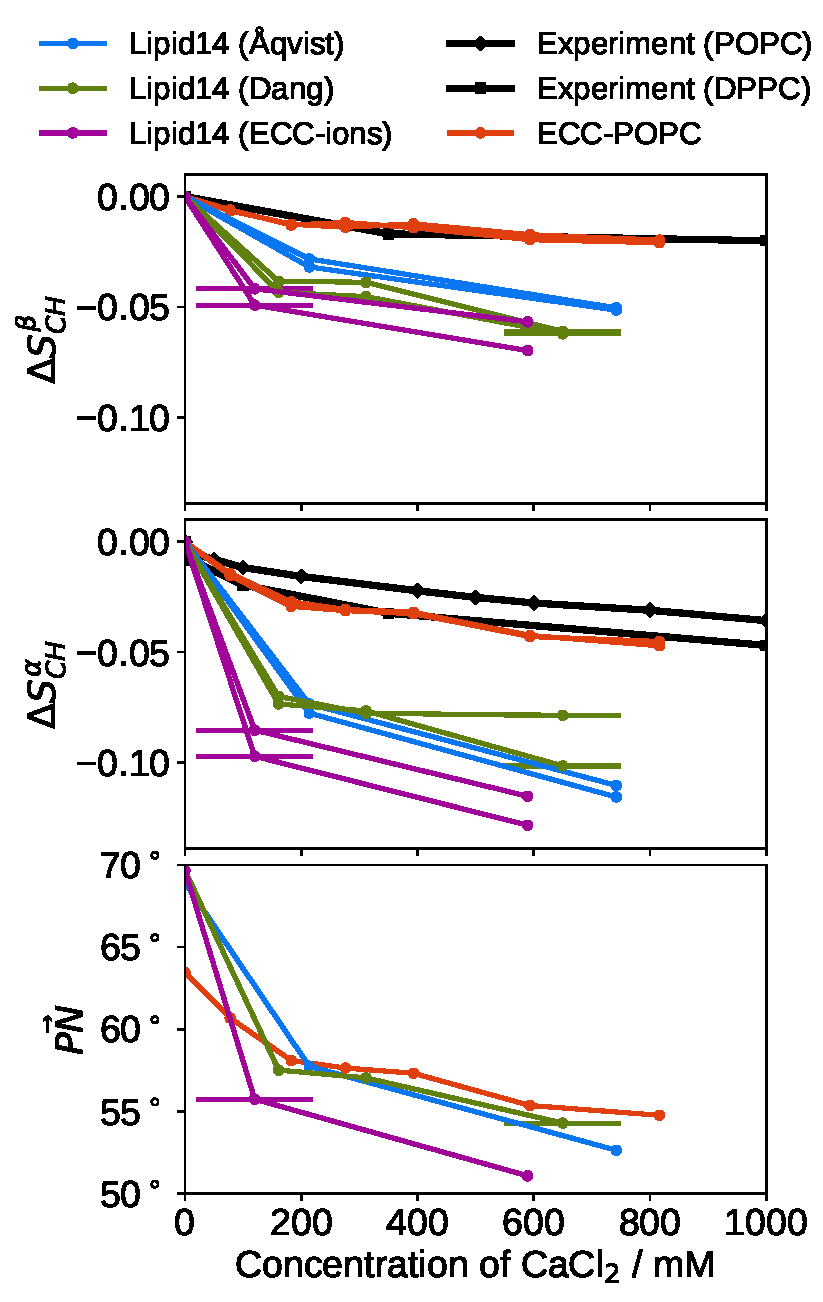
\includegraphics[width=\figwidth]{../img/ecc_popc/OrdPars-A-B-PNvec_L14-ECC-lipids_CaCl.pdf}
  \caption{\label{fig:delta_ordPar_CaCl} 
    Changes of the head group order parameters and P-N vector orientation of a POPC bilayer  
    as a function of the CaCl$_2$ concentration in bulk ($C_{ion}$) 
    from simulations at 313 K together with experimental data  
    (DPPC (323\,K) \citep{akutsu81} and POPC (313\,K) \citep{altenbach84}).  
    The error estimate for bulk concentrations is approximately 10\,mM. 
    The order of magnitude larger error in the
    simulation with Lipid14 and ECC-ions is due to unconverged bulk densities limited by the simulation box.  
    Simulation data with Lipid14 and Åqvist ion parameters at 298~K are taken directly from 
    Refs.~\citep{lipid14POPC0mMNaClfiles,lipid14POPC350mMCaClfiles,lipid14POPC350mMCaClfilesNC}. 
  } 
\end{figure} 


\begin{figure}[tbp!] 
  \centering 
  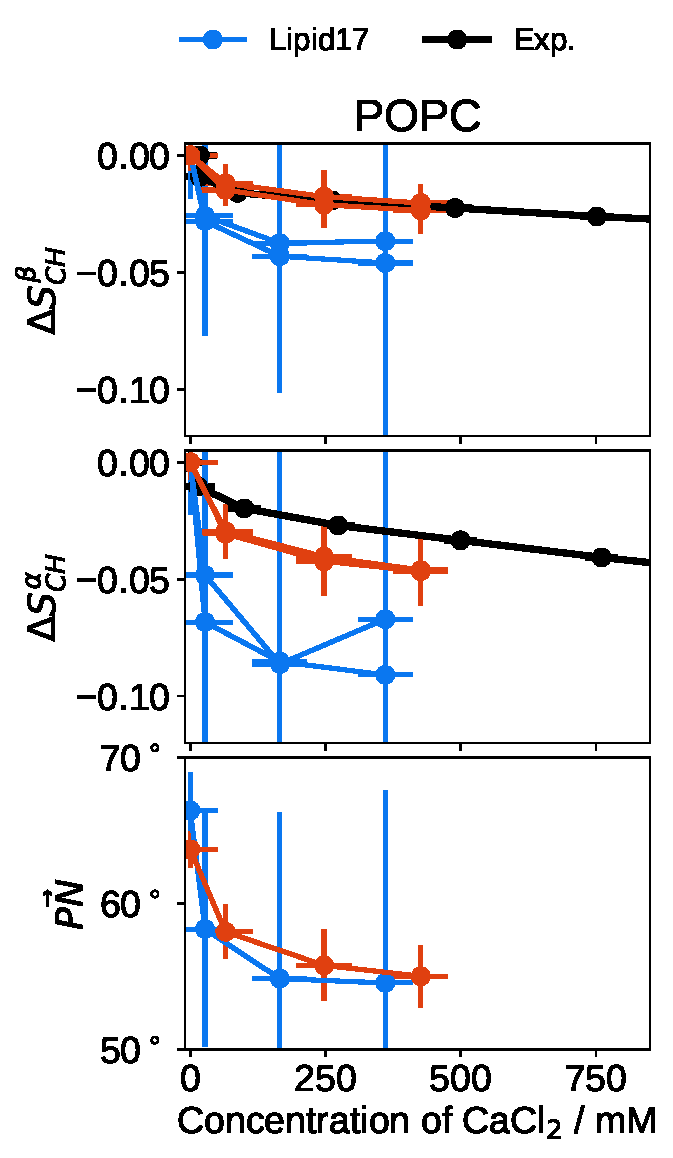
\includegraphics[width=\figwidthsmall]{../img/ecc_pops/order_parameters_changes_ecc-lip_L14_A-B-PN-COO_POPC_cacl.pdf} 
  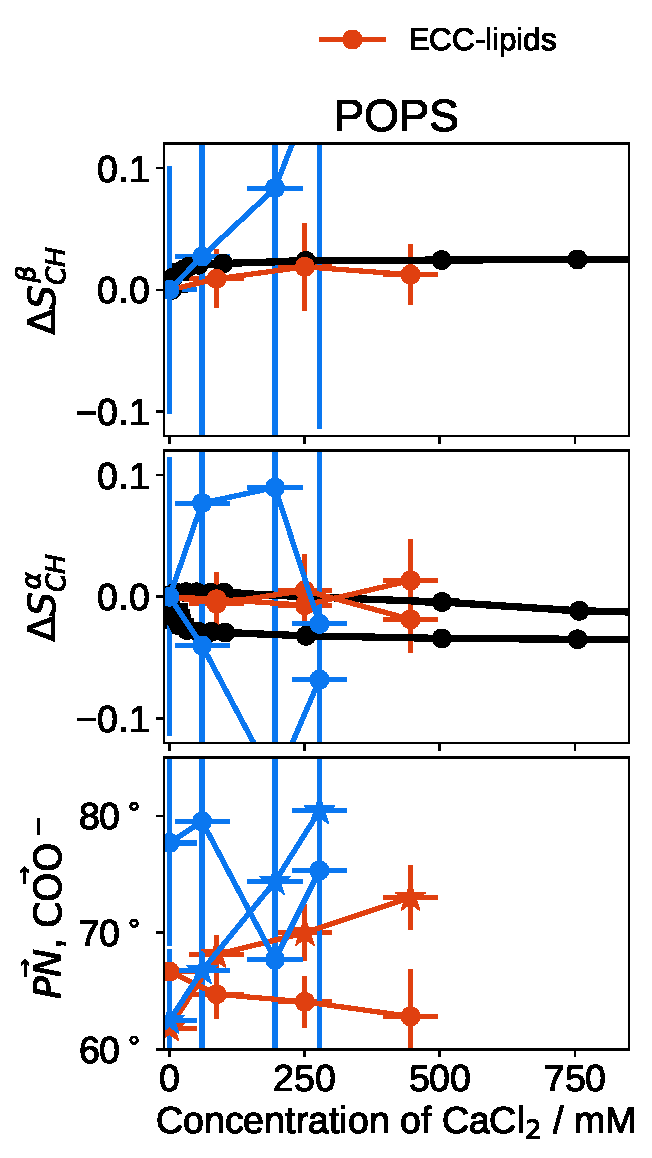
\includegraphics[width=\figwidthsmall]{../img/ecc_pops/order_parameters_changes_ecc-lip_L14_A-B-PN-COO_POPS_cacl.pdf} 
  \caption{\label{fig:delta_ordPar_CaCl_PCPS} 
    Changes of the head group order parameters $\alpha$, $\beta$ and the orientations of the carboxylate group and the P-N vector  
    of POPC (left) and POPS (right) phospholipids in a POPC:POPS 5:1 bilayer as a function of \ce{CaCl2} concentration 
    in bulk ($C_{ion}$) from simulations with different force fields and experiments at 298~K. \citep{roux90}
    The orientation of the \ce{COO^-} group is defined as 
    the connector from the $\beta$ carbon to the carbon in \ce{COO^-} (stars, bottom right). 
  } 
\end{figure} 



%%% Sum up what is to be presented briefly
%The importance of treating polarizability for interactions of phospholipids with monovalent ions was demonstrated in the previous section. 
Electronic polarization is a non-negligable contribution to the interactions of calcium even in simple aqueous solutions of \ce{CaCl2} \citep{martinek17, kohagen16, Pluharova2014}. 
In this section,
we will show the results from simulations of neutral and negatively charged phospholipid bilayers at varying \ce{CaCl2} concentrations
using the recently developed models ECC-lipids and ECC-ions \citep{melcr18, martinek17}, 
which implicitly include the effects of electronic polarization through electronic continuum correction \citep{leontyev11}. 
Validated with the concept of a lipid electrometer in section \ref{section:electrometer_exp_sim},
such implicitly polarizable models yield accurate description of 
the interaction of \ce{Ca^{2+}} with both neutral and negatively charged phospholipids. 

The changes of the head group order parameters $S^\alpha$ and $S^\beta$ from simulations and experiments 
are shown in Fig.~\ref{fig:delta_ordPar_CaCl} for a neutral POPC bialyer, 
and in Fig.~\ref{fig:delta_ordPar_CaCl_PCPS} for a negatively charged bilayer with the compostion 5\,PC:1\,PS. 
For a direct comparison and a connection to the published works by \citet{catte16, nmrlipids_proj4},
we show simulation results from Lipid17 \citep{lipid17-future} and ECC-lipids. 
It also highlights the improvements in ECC-lipids over Lipid17 arising from electronic polarization. 
%Although Lipid17 already belongs to the top-performing models in terms of the responses of the head group order parameters in those studies,  
%including electronic polarizability to form ECC-lipids improves the results even further.
The effect is probably the most striking for POPS, 
for which also the structure of a pure POPS bilayer with only counterions is dramatically improved with the augmentation. 


%%% Discuss the changes of OPs and vectors from neutral and neg. membranes
%While the changes induced by \ce{CaCl2} are \emph{qualitatively} correct for Lipid14/17, 
Using ECC-lipids, we achieve a \emph{quantitative} agreement with the changes induced by \ce{CaCl2} from experiments. 
Increasing concentrations of \ce{CaCl2} induce a systematic decrease of the order parameters $S^\alpha$ and $S^\beta$ in POPC. 
Although the total magnitude of the response of the PC head group order parameteres 
is only slightly higher in the negatively charged bilayers than in the neutral bilayers, 
the shape of the changes in the latter shows a steeper onset at low concentrations. 
This is apparently due to the presence of POPS, 
which has a higher affinity to \ce{Ca^{2+}} compared to POPC. 




\begin{figure}[htbp!] 
  \centering 
  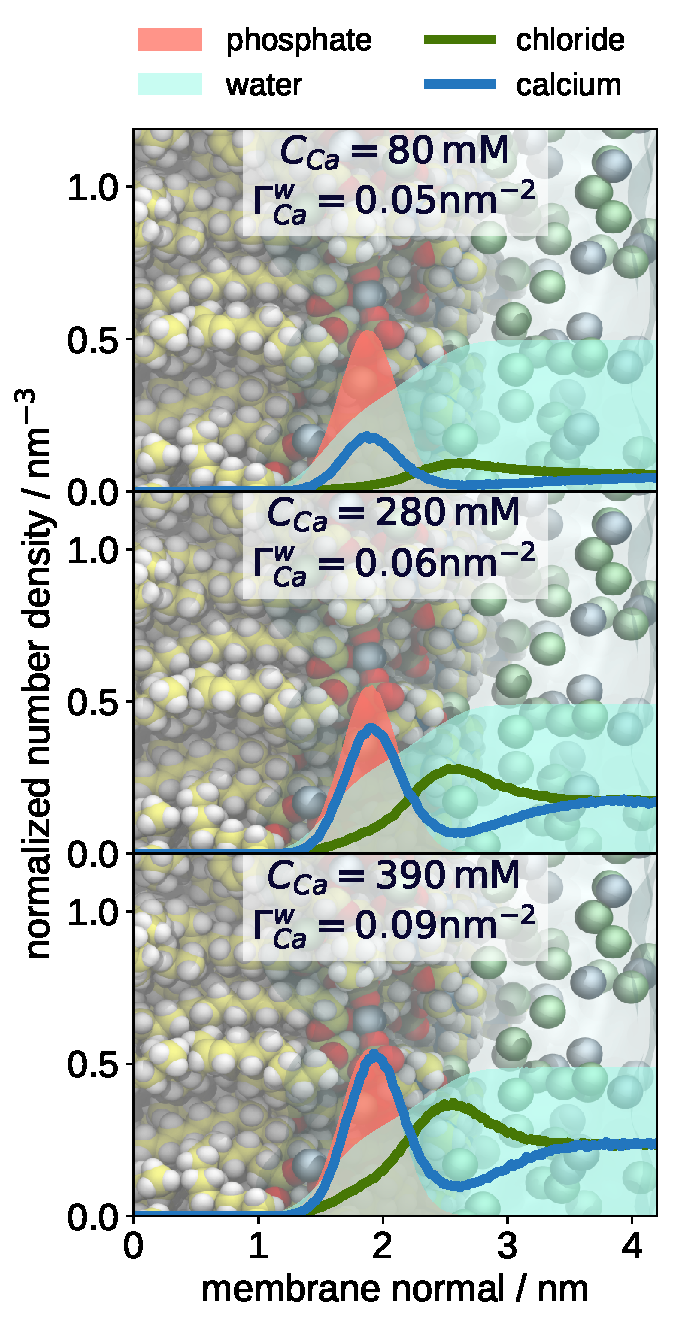
\includegraphics[width=\figwidth]{../img/ecc_popc/density_profiles_ca_cl_wat_phos_concentrations-compar.pdf} 
  \caption{\label{fig:cacl-dens} 
    Number density profiles of \ce{Ca^{2+}} and \ce{Cl^-} along the normal of the neutral POPC bilayers starting at the centre 
    for different concentrations of \ce{CaCl2} from simulations with ECC-lipids. 
    In order to visualize the density profiles with a scale comparable to the profile of \ce{Ca^{2+}},  
    the density profiles of~\ce{Cl^-} ions are divided by 2, and 
    the density profiles of phosphate groups and water are divided by 5 and 200, respectively.  
    } 
\end{figure} 


\begin{figure}[htbp!] 
  \centering 
  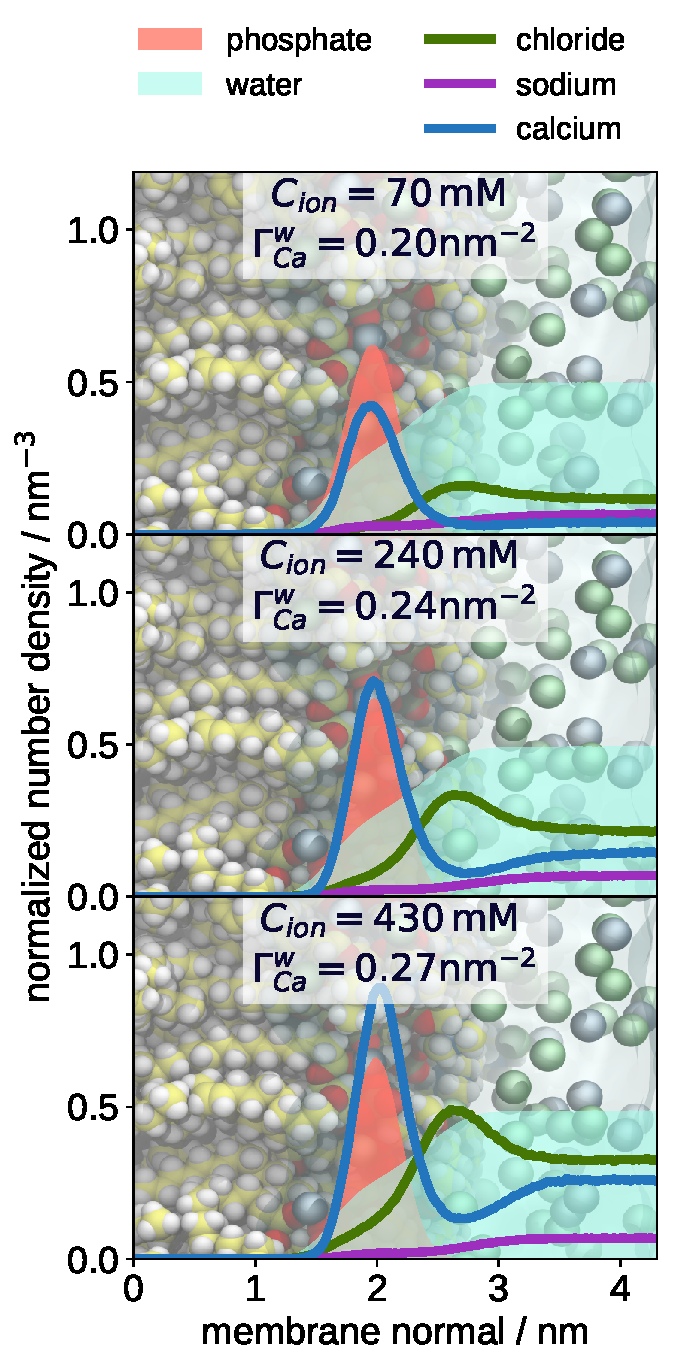
\includegraphics[width=\figwidth]{../img/ecc_pops/density_profiles_ca_na_cl_wat_phos_models-compar_1-3_CaCl2-series.pdf}
  \caption{\label{fig:cacl-dens_PCPS} 
    Number density profiles of \ce{Ca^{2+}}, \ce{Na^{+}} and \ce{Cl^-} along the normal of the membrane starting at the centre
    for the negatively charged membrane with the composition 5\,PC:1\,PS
    at various bulk concentrations of \ce{CaCl2} from simulations with ECC-lipids. 
    All profiles contain \ce{Na^+} counterions and an additional concentration of \ce{CaCl2}. 
    In order to visualize the density profiles with a scale comparable to the profile of \ce{Ca^{2+}},  
    the density profiles of~\ce{Cl^-} ions are divided by 2, and 
    the density profiles of phosphate groups and water are divided by 5 and 200, respectively.  
    } 
\end{figure} 
 





%%% Present the density profiles (different concentrations for both POPC and mixed)
The increase in the amount of bound calcium cations from pure POPC to the mixed negatively charged bilayer containing POPS
is well demonstrated using the relative surface excess, $\Gamma ^w _{Ca}$,
summarized in Table~\ref{tab:binding}. 
Distributions of \ce{Ca^{2+}}, \ce{Na^+} counterions and also \ce{Cl^-} 
are plotted in Fig.~\ref{fig:cacl-dens} for the neutral POPC bilayer, 
and in Fig.~\ref{fig:cacl-dens_PCPS} for the negatively charged bilayer. 
In contrast to \ce{KCl} or added concentrations of \ce{NaCl}, 
\ce{Na^+} counterions are substituted with \ce{Ca^{2+}} even at low concentrations of \ce{CaCl2}. 
The increasing concentration of \ce{CaCl2} and, hence, a higher amount of bound \ce{Ca^{2+}}
also attracts \ce{Cl^-} anions to the bilayer 
as can be seen from its growing density at the interface. 


%%% discuss the table with Gammas and follow up with molecular details, where do cations bind? Support with the spatial density figure
The density profiles of the ions suggest that
the dominant contribution to the binding of \ce{Ca^{2+}} to phospholipid bilayers
comes from the interactions with the phosphate groups in both POPC and POPS. 
%The population analysis also suggests 
%that the calcium cations prefer to reside in the phosphate region of the membrane. 
%Such a finding is further validated with a more detailed analysis using Markov state modeling (MSM) \citep{Pande_MSM_paper} \todoi{Add papers reviewing MSM, e.g. recent Pande's paper.}. 
%The set of states of a calcium cation 
%encompassed all possible combinations of up to three surrounding lipids. 
%In the case of PC, we used only the phosphate moitety, which forms the dominant contribution for calcium binding.
%For PS we also distinguished configurations in which calcium interacts with the carboxylate moiety. 
%All possible combinations of such states were used to build a Markov model at a lag time $25\,\mathrm{ns}$ using pyEMMA code by \citet{pyemma} \todoi{add citation for pyemma}. 
%The resulting MSM was validated using Chapman-Kolmogorov test \citep{FrankNoe_papers_MSM} \todoi{Add citation for Noe's papers on MSM, especially Chapman Kolmogorov test.}. 
%The stationary distribution of the states reveals a strong preference of the calcium cations to reside in the phosphate region of the mixed PC-PS membrane. 
%When interacting with PS, configurations with the phosphate moiety from either PC or PS dominate the population.
%Moreover, states containing interactions with the carboxylate group in PS 
%bear higher probability when interacting also with the phosphate group of the same lipid or other lipids. 
This is also reflected in the shift of the mean orientation 
of the \ce{COO^-} group from $62^\circ$ to $73^\circ$ (420~mM \ce{CaCl2})
which was measured as the connector of the carbon atoms 
forming the bond between the group and the $\beta$-carbon of the phospholipid. 
The interactions of the carboxylate group in PS with calcium and other phosphate groups
shed light into the qualitatively different response of the head group order parameters $\alpha$ and $\beta$ in PS compared to PC 
(see Figs.~\ref{fig:delta_ordPar_CaCl} and~\ref{fig:delta_ordPar_CaCl_PCPS}). 
We find that the complex response of the head group order parameters of POPS 
is affected by the confomational changes of the carboxylate group,
which is attracted more towards the phosphate region, 
where the calcium cations dominantly bind. 
This is also very likely the reason, 
why the magnitude of the P-N vector change in POPS is diminished compared to POPC, 
which is not restrained by an additional cation binding group like \ce{COO^-} in POPS. 


Further detailes about the interactions of \ce{Ca^{2+}} with varoius moieties in POPC or POPS
were obtained by counting contacts between the cations and the oxygen atoms of the lipids
similarly as was done in \cite{melcr18}. 
The threshold for counting a contact was set to $0.3\,\mathrm{nm}$, 
which encompasses the first peak of the radial distribution function between the cations and the oxygen atoms of the lipids. 


\begin{table}[tb!] 
\centering
  \caption{Bulk concentrations, $C _{ion}$, and molar fractions, $C' _{ion}$, of Ca$^{2+}$;
           relative surface excess of calcium with respect to water ($\Gamma_{Ca}^{\rm water}$); 
           and percentages of the population 
           of bound Ca$^{2+}$ to various moieties 
           in a neutral membrane composed of POPC
           and in a negatively charged membrane with the compostion 5\,PC:1\,PS.
           \label{tab:binding}} 
  \begin{tabular}{ l | c c } 
	                     &  5\,POPC:1\,POPS &  POPC   \\
	\hline
	$C _{ion}\,/\,\mathrm{mM}$  &  $240\pm 10 $  &  $280\pm 10 $  \\
	$C'_{ion}\,/\,\mathrm{mM}$  &  $400\pm 10 $  &  $350\pm 10 $  \\
	$\Gamma_{Ca}^{\rm water}\, / \,\mathrm{nm}^{-2}$  &  $0.24 \pm 0.01 $  &  $0.06 \pm 0.01 $  \\
	\hline
                             &  \multicolumn{2}{c}{ } \\
        interacting moiety   &  \multicolumn{2}{c}{percentage of bound \ce{Ca^{2+}} } \\
	\hline
	     PC              &   59   &  100   \\
	     PO$_4$    in PC &   41   &   67   \\
	     carbonyls in PC &   <1   &   ~1   \\
	\hline
	     PS              &    8   &        \\ 
	     PO$_4$  in PS   &    2   &        \\
	     COO$^-$ in PS   &    4   &        \\
	     carbonyls in PS &   <1   &        \\
	\hline
	both PC and PS       &   33   &        \\
  \end{tabular} 
\end{table} 




\begin{figure}[tb!] 
  \centering 
  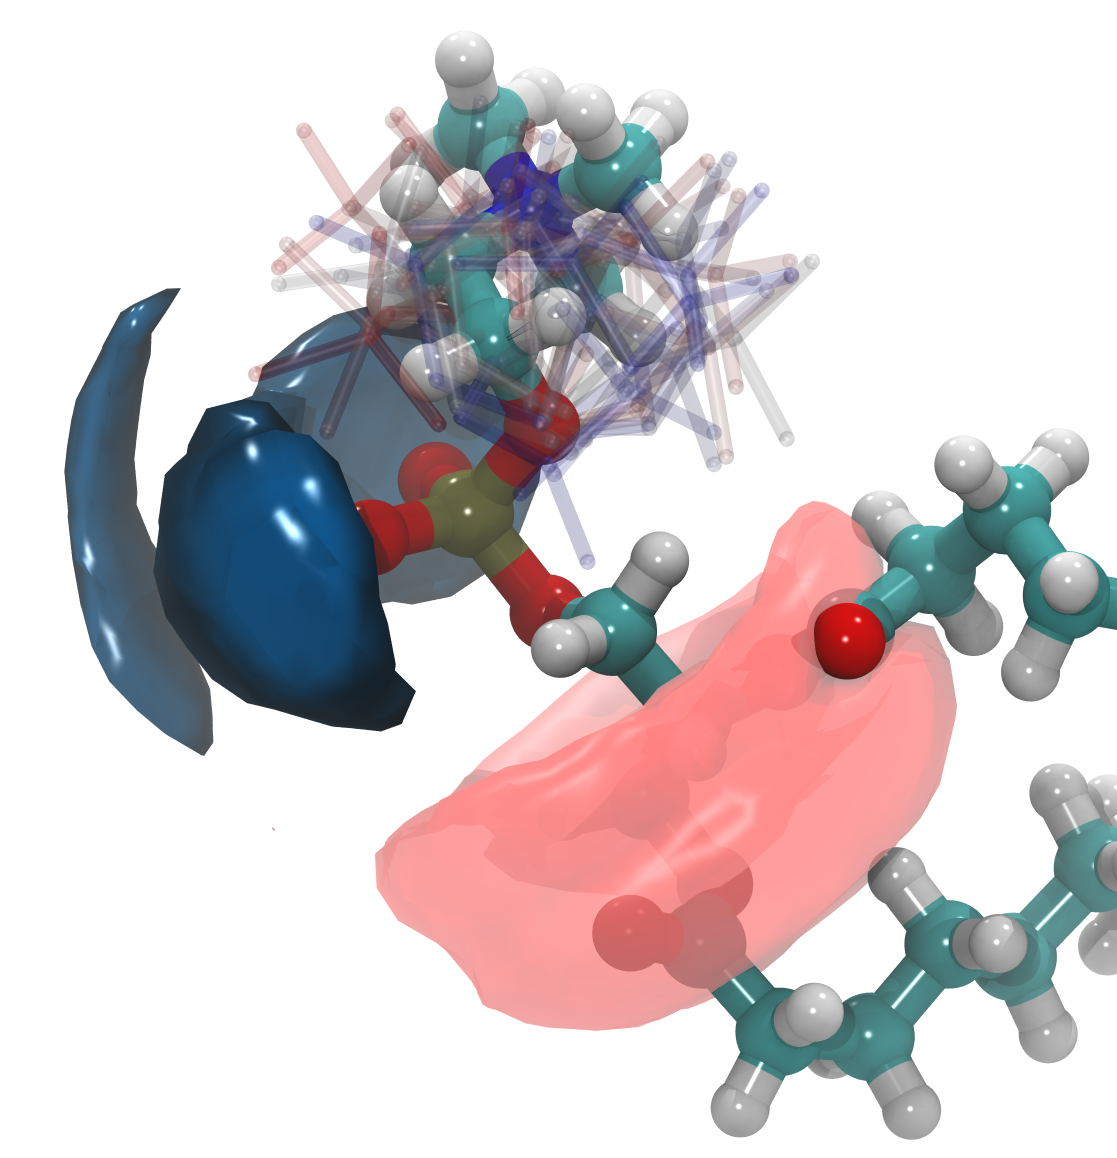
\includegraphics[width=\figwidth]{../img/ecc_popc/isocontours_r37_ca_O-carb.png} 
  \caption{\label{fig:volmaps} 
    Isocontours of spatial number density of \ce{Ca^{2+}} (dark blue, 0.001~Å$^{-3}$) 
    and POPC carbonyl oxygen atoms (light semi-transparent red, 0.008~Å$^{-3}$, all POPC lipids contribute). 
    Calcium cations localize mostly around phosphate oxygens (oxygens red, phosphorus bronze).
    Interactions with carbonyl oxygens is less likely than with phosphate oxygens, 
    and it is contributed more by other neighbouring phospholipids than by the same lipid. 
    Transparent structures are shown to depict the variability of choline configurations 
    (colour warps from red to blue along the simulation time). 
    The number density was evaluated for each lipid, 
    after its structural alignment using only phosphate group.
    MDAnalysis \citep{mdanalysis2011} library was used for 
    the calculations of the structural alignment and the spatial number density. 
    VMD \citep{hump96} was used for visualisation. 
    Carbon atoms are depicted in cyan, hydrogen atoms in white, oxygen atoms in red, nitrogen in blue.
  } 
\end{figure} 



The percentages of the populations of membrane-bound calcium cations for various membrane moieties 
are summarized in Table~\ref{tab:binding}.
Even though the negatively charged membrane contains only 18\% of POPS, 
approximately 41\% of the total population of bound calcium cations is in contact with PS lipids
with 8\% bound only to them. 
This corroborates the intrinsincally higher affinity of PS lipids to calcium cations compared to neutral PC lipids. 
POPC interacts with the calcium cations almost entirely through its phosphate group 
in both neutral and negatively charged membranes, 
which is visualized using probability density isocontours in Fig.~\ref{fig:volmaps}.
Interactions of \ce{Ca^{2+}} with carbonyl groups are also present, 
however, they are always accompanied by interactions with pohsphate groups. 
%but a very small negligable amount much below 1\%. 



\begin{figure}[tb!] 
  \centering 
  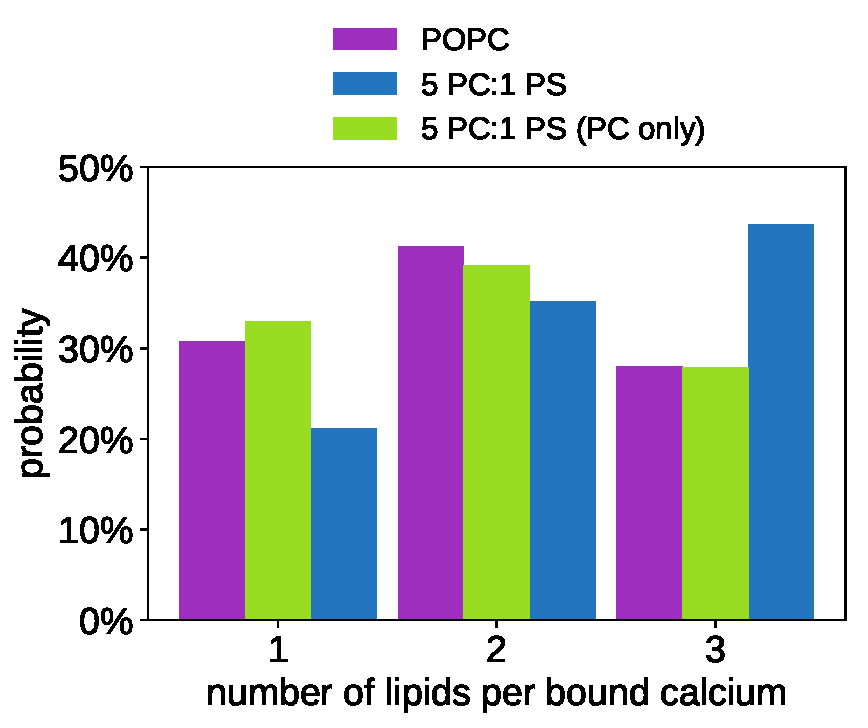
\includegraphics[width=\figwidth]{../img/stoichiometry_CaCl2_comparison_Ecc-lipids_PC-vs-PCPS.pdf} \\ 
  \caption{\label{fig:cacl_complexes} 
      Relative probabilities of existence of \ce{Ca^{2+}} complexes 
      with a certain number of lipids.  
      All lipids were taken into account with the exception of the complexes in light green and orange, 
      for which we counted only contacts with POPC resp POPS from the mixed 5\,PC:1\,PS negatively charged bilayer. 
      The calculated probabilities of the calcium-lipid complexes also reflect only POPC (light green) resp POPS (orange). 
      Probabilities were taken from simulations with comparable bulk concentrations of calcium around 250~mM. 
      Clusters of four or more lipids were not observed in either membrane. 
  } 
\end{figure} 




Relative probabilites of \ce{Ca^{2+}} complexes with a certain number of lipids are presented in Fig.~\ref{fig:cacl_complexes}. 
Calcium cations that are bound only to PC in the mixed bilayer with PS 
behave similarly as in the pure PC bilayer
maintaining comparable probabilities for clustering one, two, or even three PC lipids together. 
In contrast, PS lipids prefer 1:1 ratio with \ce{Ca^{2+}},
which may also be due to their low molar fraction in the the mixed bilayer. 
In total, however, the negatively charged membrane has its stoichiometry 
shifted towards complexes with three phospholipids and one calcium. 
This is obviously due to the presence of POPS, 
which also contributes to the pre-formed one- and two-membered clusters of POPC. 
Clusters of four or more lipids were not observed in either membrane. 

%This is also reflected in the increased probability 
%of a single phospholipid interacting with two \ce{Ca^{2+}} cations 
%compared to the neutral POPC bilayer, 
%where such a probability is almost negligable. 
% Not shown through numbers, however, I have the plots to back it. 









 
 
 





%\todo{Stationary distribution: Make a figure documenting the populations of bound \ce{Ca^{2+}} cations (like I have in the presentation) that would accompany Table \ref{tab:Ca_binding_PCPS}. 
%This will roughly correspond to the PC stoichiometry plot \ref{fig:cacl_complexes}. }




\begin{figure}[tb!]
  \centering
  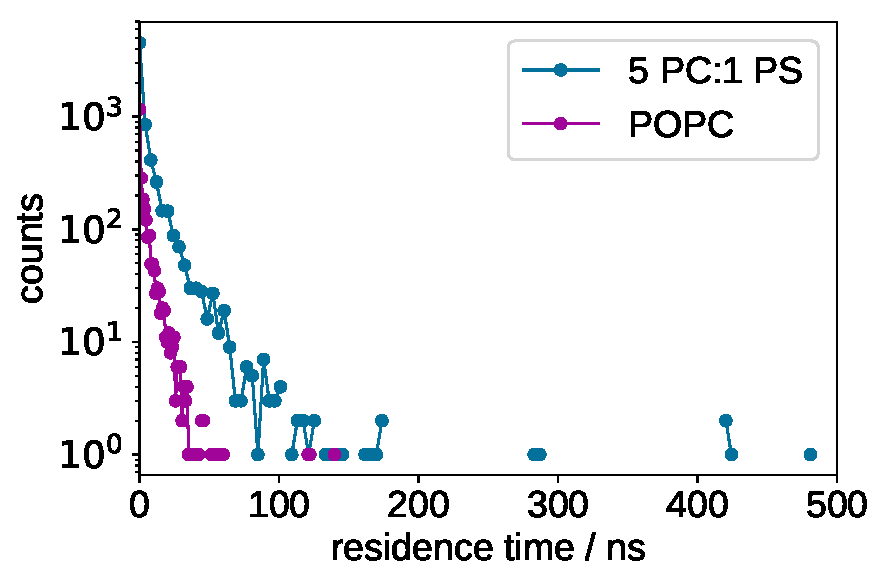
\includegraphics[width=\figwidth]{../img/histogram_bound_times_26CaCl2_comparison_PC-PCPS.pdf}
  \caption{\label{fig:hist_residence_times}
   Histograms of residence times of \ce{Ca^{2+}} 
   in a neutral membrane composed of POPC (orange)
   and in a negatively charged membrane with the compostion 5\,PC:1\,PS (blue)
   from simulations with ECC-lipids and ECC-ions.
   The simulation with the neutral membrane has a bulk concentration of calcium $C_{ion} = 280\mathrm{mM}$, 
   the simulation with the negatively charged membrane has a bulk concentration of calcium $C_{ion} = 240\mathrm{mM}$. 
   In the simulation with the neutral membrane, 
   90\% of the residence times of calcium cations are
   shorter than $60\,\mathrm{ns}$, % exactly $53\,\mathrm{ns}$                                                                          
   with the longest observed residence time being $141\,\mathrm{ns}$. 
   In the simulation with the negatively charged membrane, 
   90\% of the residence times of calcium cations are
   shorter than $200\,\mathrm{ns}$, % exactly $53\,\mathrm{ns}$                                                                          
   with the longest observed residence time being $485\,\mathrm{ns}$. 
   }
\end{figure}


Timescales associated with the binding of calcium cations from solution to the membrane
are plotted for each binding event as a histogram in Fig.~\ref{fig:hist_residence_times}. 
Using these plots, we can estimate that 90\% of the residence times of any calcium cation 
will be lower than $60\,\mathrm{ns}$ for pure POPC neutral bilayer 
and shorter than $200\,\mathrm{ns}$ for the mixed 5\,PC:1\,PS negatively charged bilayer. 
The longest observed residence times in the simulations were $141\,\mathrm{ns}$ for the neutral membrane 
and $485\,\mathrm{ns}$ for the negatively charged membrane. 
Both estimates of the residence times come from simulations with comparable concentrations of around $250\mathrm{mM}$;
the simulation with the neutral membrane has a bulk concentration of calcium $C_{ion} = 280\mathrm{mM}$, 
whereas the simulation with the negatively charged membrane has a bulk concentration of calcium $C_{ion} = 240\mathrm{mM}$. 

In summary, the results from ECC-lipids suggest 
that the exchange of calcium between the POPC bilayer and the solvent 
occurs at the order of $\sim$10--100~ns, 
which is significantly faster than observed in simulations 
with other presently available non-polarizble models of lipids and ions~\citep{javanainen17, catte16}. 
Our results suggest 
that simulation trajectories with a characterisitc length of several hundreds of nanoseconds 
are necessary to cpature the binding of calcium to neutral POPC bilayers 
in equilibrium when more realistic \emph{polarizable} force fields are used. 
Interestingly enough, almost an order of magnitude longer simulations
are required for the negatively charged bilayers. 

 
%In addition to such estimates of the time scales, we used the Markov model on top of the simulation with the negatviely charged mixed bilayer
%to calculate the time of the mean first passage of calcium from solution to the membrane (and in reverse) resulting in $55\,\mathrm{ns}$  ($165\,\mathrm{ns}$). 

%\todo{Fluxes: committor analysis, dominant fluxes (table and figure)}
%From the spectrum of the transition matrix, we also observe that 
%the slowest transitions are associated with the binding to two or three phosphate moieties from either PC or PS,
%which are also among the states with the highest probabilities.
%The net fluxes of calcium cations from solution to such states also form a large contribution to the total flux ($\approx 45\%$). 
%\todo{Make a table and a figure of the state probabilities and fluxes to support this statement.}. 
%Analysis of the possible binding pathways of calcium cations to the negatively charged mixed bilayer 
%reveal that the cations mostly enter the membrane bound states directly from solution 
%without complicated transitions at the time scales of the order of the lag time of the Markov state model, $25\,\mathrm{ns}$. 

